\subsection{FRASP}

\textbf{FRASP (Functional Reactive Approach to Self-organisation Programming)}\footnote{\url{https://github.com/cric96/distributed-frp}}
is a new open-source aggregate computing framework for the Scala programming
language, currently under active research.

FRASP draws inspiration from \ac{ScaFi}, sharing many similarities. The key
distinction lies in the implemented execution model: the former adopts a novel
functional reactive execution model, leveraging the Sodium library, as opposed
to the round-based execution model of the latter, common in aggregate computing
\cite{FRASP}.

The motivation behind FRASP is to provide for some of the shortcomings of the
round-based execution model, including \textit{periodic computation},
\textit{complete re-computation} and \textit{redundant message exchanges}.
Indeed, the benefits of adopting the execution model of FRASP for aggregate
computing are the following:
\begin{itemize}
  \item \textit{Event-driven computation}: in a device, computation is driven
        by relevant changes in its perception of the environment (e.g.
        sensors, neighbor data). In other words, computation is performed only
        when required.
  \item \textit{Independent scheduling of sub-computations}: when a device
        detects a change in its context, only the dependent sub-computations
        of its programs are re-computed. In other words, full re-computations
        of an aggregate specification are avoided when possible.
  \item \textit{Minimal communication}: a device only broadcasts its exports
        upon relevant changes, avoiding further message exchanges after the
        aggregate reaches a stable configuration. In other words, redundant
        computation caused by repeated messages is avoided.
\end{itemize}

In FRASP, computational fields are reified into Sodium's \texttt{Cell}s, which
neatly capture their time-varying nature. Like \ac{FRP}, a specification is the
configuration of a computational graph, which tracks the dependencies between
computational fields and manages the propagation of change automatically.

Computational fields are initialized by \texttt{Flow}s, which model
sub-computations in an aggregate specification and are first-class citizens in
FRASP. The purpose of \texttt{Flow}s is to defer the construction of the
computational graph until the devices of the aggregate network are initialized,
which is required to express dependencies related to their neighbors and
sensors. In addition, \texttt{Flow}s also keep track of their position inside
the FRASP specification, building the abstract syntax tree used for alignment.

The semantics of FRASP (Listing \ref{listing:frasp-language}) faithfully
resembles the semantics of field calculus, while also sharing common constructs
with \ac{ScaFi}. However, since computational fields have been reified,
additional operators are required to adapt values yielded by plain Scala
expressions to the language constructs, namely \texttt{constant} for values and
\texttt{lift} for operators (\textit{lifting}).

The main difference with the field calculus semantics is the \texttt{loop}
construct, replacing the \texttt{rep} construct. The \texttt{loop} construct
implements the evolution of a computational field over time as a (cyclic)
self-dependency within the computational graph of a FRASP specification, rather
than relying on the concept of computation round. Indeed, the previous state of
a device is computed through self-alignment, leveraging the fact that every
device is a neighbor of itself.

\begin{lstlisting}[
  language=Scala,
  caption={The core constructs of the FRASP language, represented as a trait,
  abstracting over the actual organization within FRASP.},
  captionpos=b,
  label={listing:frasp-language}
]
trait FraspLanguage:
  // field calculus
  type Flow[V]
  def constant[V](value: V): Flow[V]
  def lift[A, B, C](a: Flow[A], b: Flow[B])(operator: (A, B) => C): Flow[C]
  def loop[V](init: V)(evolve: Flow[V] => Flow[V]): Flow[V]
  def nbr[V](cond: Flow[Boolean])(th: Flow[V])(el: Flow[V])
    : Flow[NeighboringValue[V]]
  def branch[V](cond: Flow[Boolean])(th: Flow[V])(el: Flow[V]): Flow[V]

  // platform interactions
  def mid: Flow[DeviceId]
  def sensor[V](name: LocalSensorId): Flow[V]
  def nbrSensor[V](name: NeighborSensorId): Flow[NeighboringValue[V]]

  // derived operations
  def mux[V](cond: Flow[Boolean])(th: Flow[V])(el: Flow[V]): Flow[V]
  def share[V](init: Flow[V])(evolve: Flow[NeighboringValue[V]] => Flow[V])
    : Flow[V]
\end{lstlisting}



FRASP also provides a basic simulator implementing its reactive execution model
(Figures \ref{figure:frasp-simulation} and
\ref{figure:frasp-simulation-example}). On an abstract level, the simulator
operates in two phases:
\begin{itemize}
  \item \textbf{Configuration}: accept a FRASP specification, which describes
        the configuration of a computational graph, and an environment, which
        describes the devices of the aggregate and their neighboring relations
        (e.g. based on proximity);
  \item \textbf{Execution}: create the devices and build the computational
        graph of the aggregate, based on the FRASP specification. In doing so,
        the simulator establishes the dependency chains from the perceptions of
        each device (e.g. neighbor and environmental data) to its exports and
        from its exports to the neighbor data perceived by its neighbors.
        As soon as the graph is built, the \textit{input nodes}\footnote{
          a node initialized by a leaf \texttt{Flow} in the abstract syntax
          tree of a FRASP specification: either \texttt{constant}, \texttt{mid},
          \texttt{sensor}, \texttt{nbrSensor} or \texttt{loop}, as they do not
          require other \texttt{Flow}s in input.
        } of the computational graph will propagate their initial value to all
        their dependents, then the computation is carried on automatically by
        the underlying \ac{FRP} engine indefinitely.

        Since non-trivial specifications for aggregate computing include cyclic
        dependencies in the computational graph, additional measures must be
        taken to avoid the indefinite propagation of non-relevant changes (e.g.
        redundant messages). In particular, FRASP applies the FRP calming
        pattern to all nodes when building a computational graph, allowing
        self-stabilizing specifications to eventually reach a stable state, in
        which events are no longer propagated in the aggregate until the next
        change in the environment. Note that the execution is still indefinite
        even after reaching a stable state, since it is always possible for an
        event to happen in the future, however, no propagation of changes
        implies no consumption of computational resources (i.e. the aggregate
        keeps waiting for an event to occur).
\end{itemize}

\begin{figure}[!ht]
  \centering
  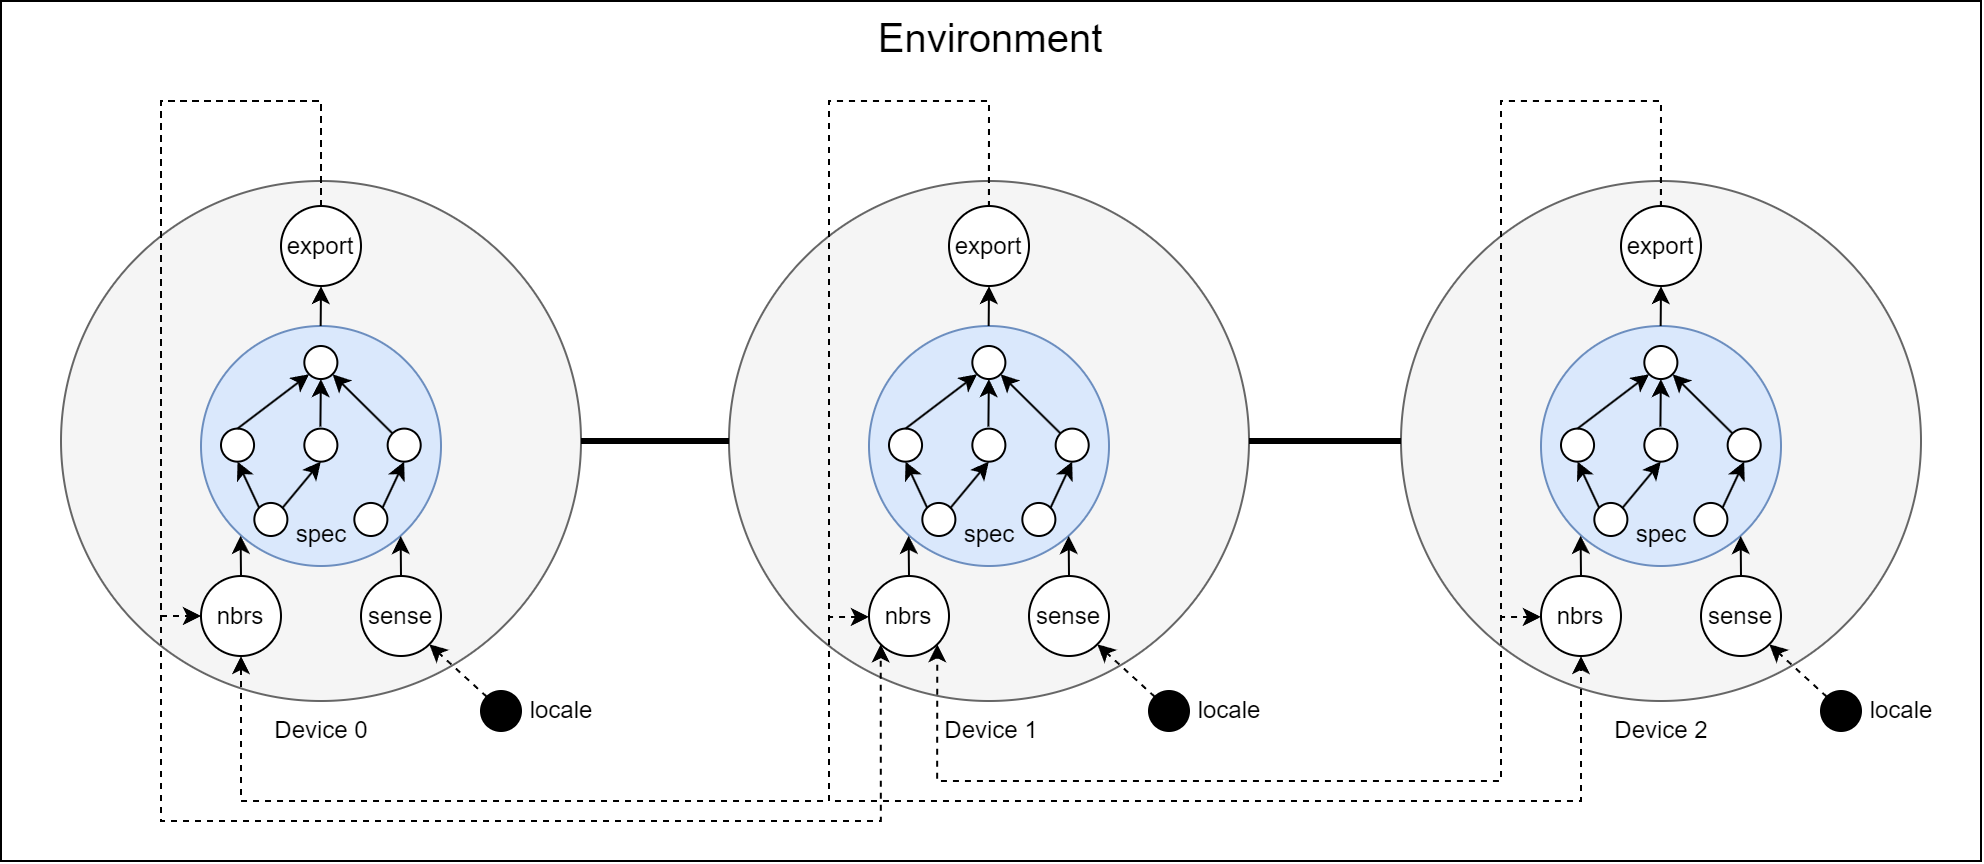
\includegraphics[width=1\textwidth]{resources/figures/frasp-simulation.png}
  \caption{
    The reactive execution model of FRASP. In the diagram, there are three
    devices (\textit{grey circles}), each configured with an aggregate
    specification (\textit{blue circles}). For each device, the input of the
    aggregate specification is neighboring (\textit{nbrs}) and local
    environmental data (\textit{sense}); the output is the export that needs to
    be broadcast to neighbors (\textit{export}). The figure also shows internal
    (\textit{solid arrow}) and external (\textit{dashed arrow}) dependencies in
    the computational graph.
  }
  \label{figure:frasp-simulation}
\end{figure}

\begin{figure}[!ht]
  \centering
  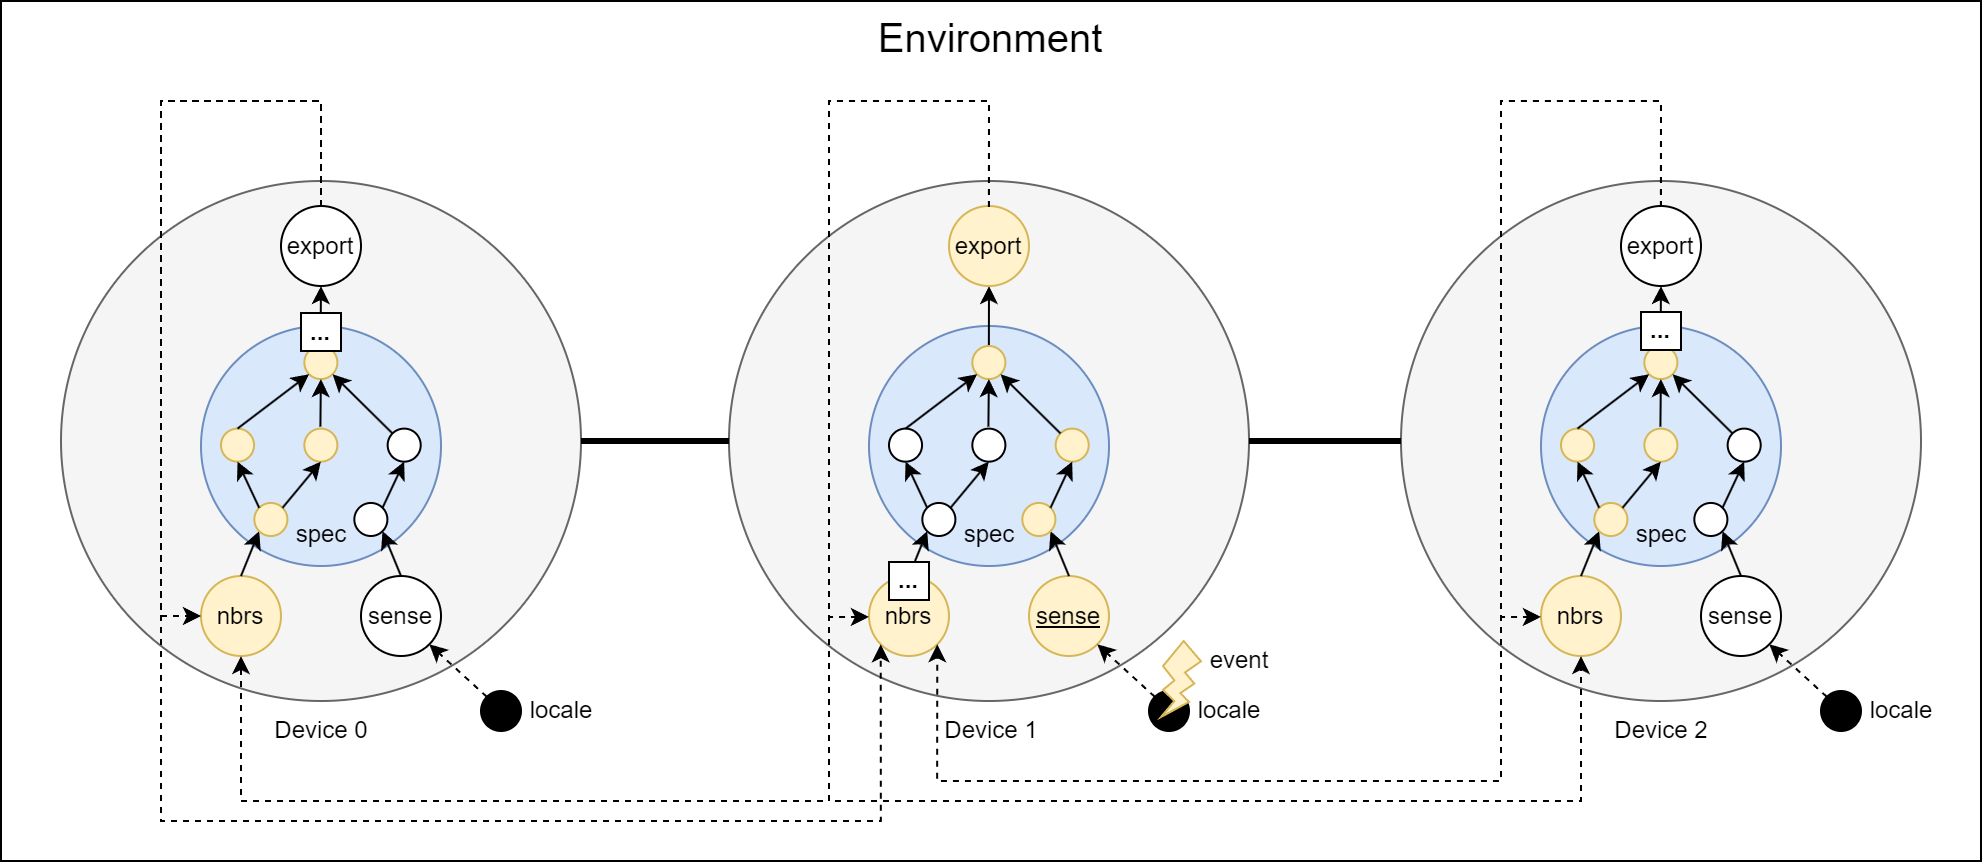
\includegraphics[width=1\textwidth]{resources/figures/frasp-simulation-example.png}
  \caption{
    An example of propagation of change in the execution model of FRASP. The
    local environment of device 1 changed, causing changes to all its
    dependents. The three dots indicate that the change would continue to
    propagate afterward following the graph dependencies. Note how the
    propagation of change would carry on indefinitely in any cyclic graph
    without proper measures.
  }
  \label{figure:frasp-simulation-example}
\end{figure}

Since this project contributes to the implementation of FRASP, a brief overview
of its architecture is due. Internally, FRASP is organized into the following
three layered modules (Figure \ref{figure:frasp-modules}):
\begin{itemize}
  \item \texttt{frp}: provide extensions and abstractions over the \ac{FRP}
        engine on which the framework depends.
  \item \texttt{core}: provide the model and implementation of the FRASP
        specification, as illustrated previously in Listing
        \ref{listing:frasp-language}.
  \item \texttt{simulation}: provide a basic simulator for running aggregate
        specifications over a network of devices.
\end{itemize}
\begin{figure}[h]
  \centering
  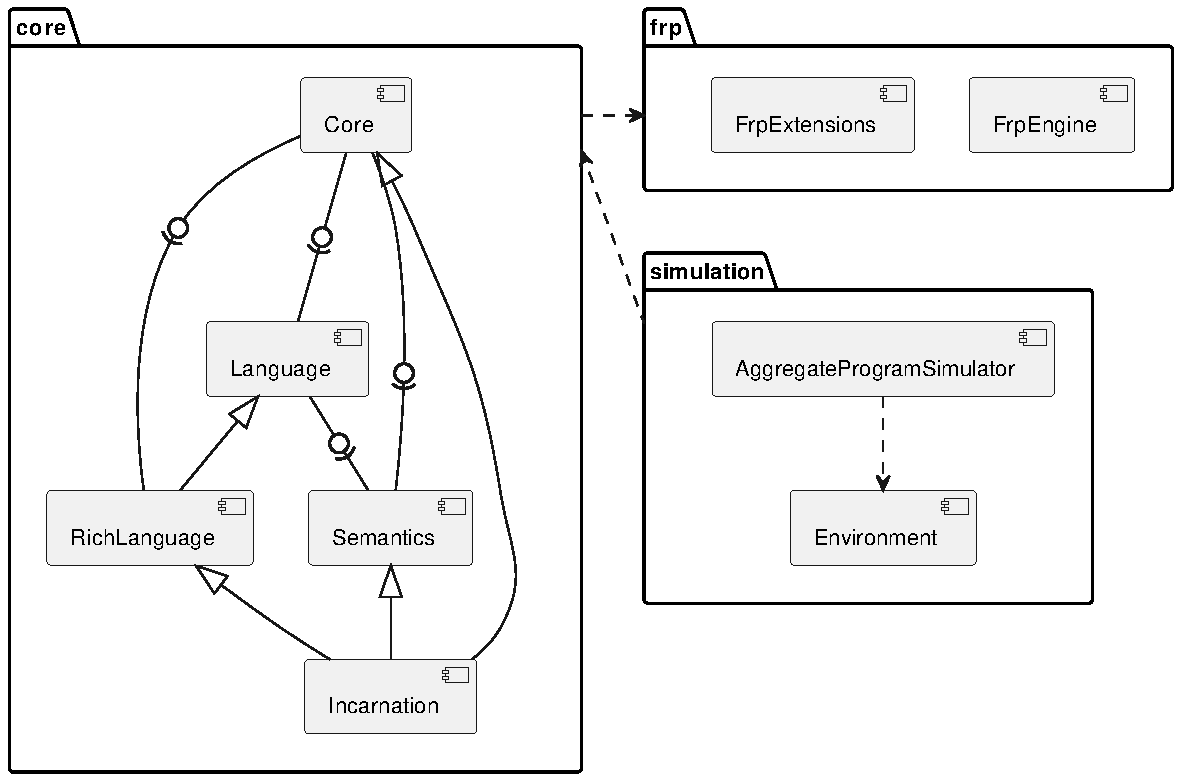
\includegraphics[width=1\textwidth]{resources/figures/frasp-modules.pdf}
  \caption{The architecture of FRASP \cite{FRASP}.}
  \label{figure:frasp-modules}
\end{figure}

The contributions of this project concern mostly the \texttt{frp} and
\texttt{simulation} modules. More details will be provided in the following
chapters as needed.
